\subsection{Three dimensional uniform dataset}

The three dimensional uniform dataset (that corresponds to the RGB color cube) is an interesting low dimensional case that requires a dimensionality reduction (from dimension 3 to 2). Since we used a uniform distribution this means the dataset is a dense three dimensional manifold that needs to be mapped to a two dimensional manifold which is known not to have an optimal solution. However, this difficulty can be partially alleviated using a loose topology in the RSOM. This is made possible by using a 2-neighbours induced topology as shown in figure \ref{fig:3D-uniform:results}A. This weak topology possesses several disconnected subgraphs that relax the constraints on the neighborhood of the BMU (see figure \ref{fig:topology-influence} in the supplementary section for the influence of neighborhood on the self-organization). This is clearly illustrated in figure \ref{fig:3D-uniform:results}B where the Voronoi cell of a neuron has been painted with the color of its codeword. We can observe an apparent structure of the RGB spectrum with some localized ruptures. To test for the completeness of the representation, we represented the position of six fundamental colors (C - white (1,1,1), D - black (0,0,0), E - yellow (1,1,0), F - red (1,0,0), G - green (0,1,0) and H - blue (0,0,1)) along with their associated distance maps after learning.

Furthermore, we performed the persistent homology to identify important topological features in the
input space and investigate how well the SOM and RSOM captured those features. Figures
\ref{fig:3D-uniform:analysis}A, B, and C show the persistent barcodes for the input space, SOM, and 
RSOM, respectively. We can see how the RSOM (panel C) captures more $H1$- and $H2$-homological properties
(since there are more persistent line segments, orange and green lines). The SOM (panel B) seems to capture
some of those features as well but they do not persist as long as they in the case of RSOM. The persistence 
diagrams of input, SOM and RSOM are shown in figures~\ref{fig:3D-uniform:analysis} D, E, and F, respectively.
These figures indicate that the RSOM has more persistent features (orange and green dots away from the diagonal
line) than the regular SOM.
The Bottleneck distance between the persistence diagrams of input space and those of SOM and RSOM reveals
that the SOM's persistence diagram is slightly closer to the input space's one for both the $H0$ (SOM: $0.00035$,
RSOM: $0.0007$), $H1$ (SOM: $0.006$, RSOM: $0.007$), and $H2$ (SOM: $0.0062$, RSOM: $0.0057$). Despite the 
fact that the bottleneck distances show that 
regular SOM's persistent diagram is closer to input space's one, the barcodes diagrams indicate that the RSOM 
captures more persistent topological features suggesting that RSOM preserves in a better way the topology of the
input space. Furthermore, the RSOM seems to capture better the higher dimensional topological features since the 
Bottleneck distances of $H2$-homological features are smaller for the RSOM than for the SOM.

% For the three-dimensional experiment we draw 50,000 three-dimensional points from a uniform distribution $\mathcal{U}([0, 1]\times [0, 1]\times [0, 1])$ (the cloud points form a cube in $\mathbb{R}^3$). The map is a two-dimensional manifold and thus the required task it to map the three-dimensional vectors  to the two-dimensional neural space. Once again we place the neurons on the two-dimensional neural space based on the sampling of a blue noise distribution and the induced topology is illustrated in Figure~\ref{fig:3D-uniform:results}A. The learning algorithm runs for $25000$ epochs over the three-dimensional vectors and after convergence we  obtain the map with the prototypes shown in Figure~\ref{fig:3D-uniform:results}B. Each color represents a different face of the three-dimensional cube (a cube has six faces so we obtain mainly six colors) and we observe that the SOM has mapped the three-dimensional cube on a two-dimensional neural space. The continuity and grouping of the colors indicates that the receptive fields of the neurons have been established properly. We illustrate this phenomenon in panels~\ref{fig:3D-uniform:results}C-H,  where the response of six different neurons (see the annotation in panel~\ref{fig:3D-uniform:results}B). The dark blue color indicates values close to zero and the yellow color represents values close to one.


\begin{figure}
  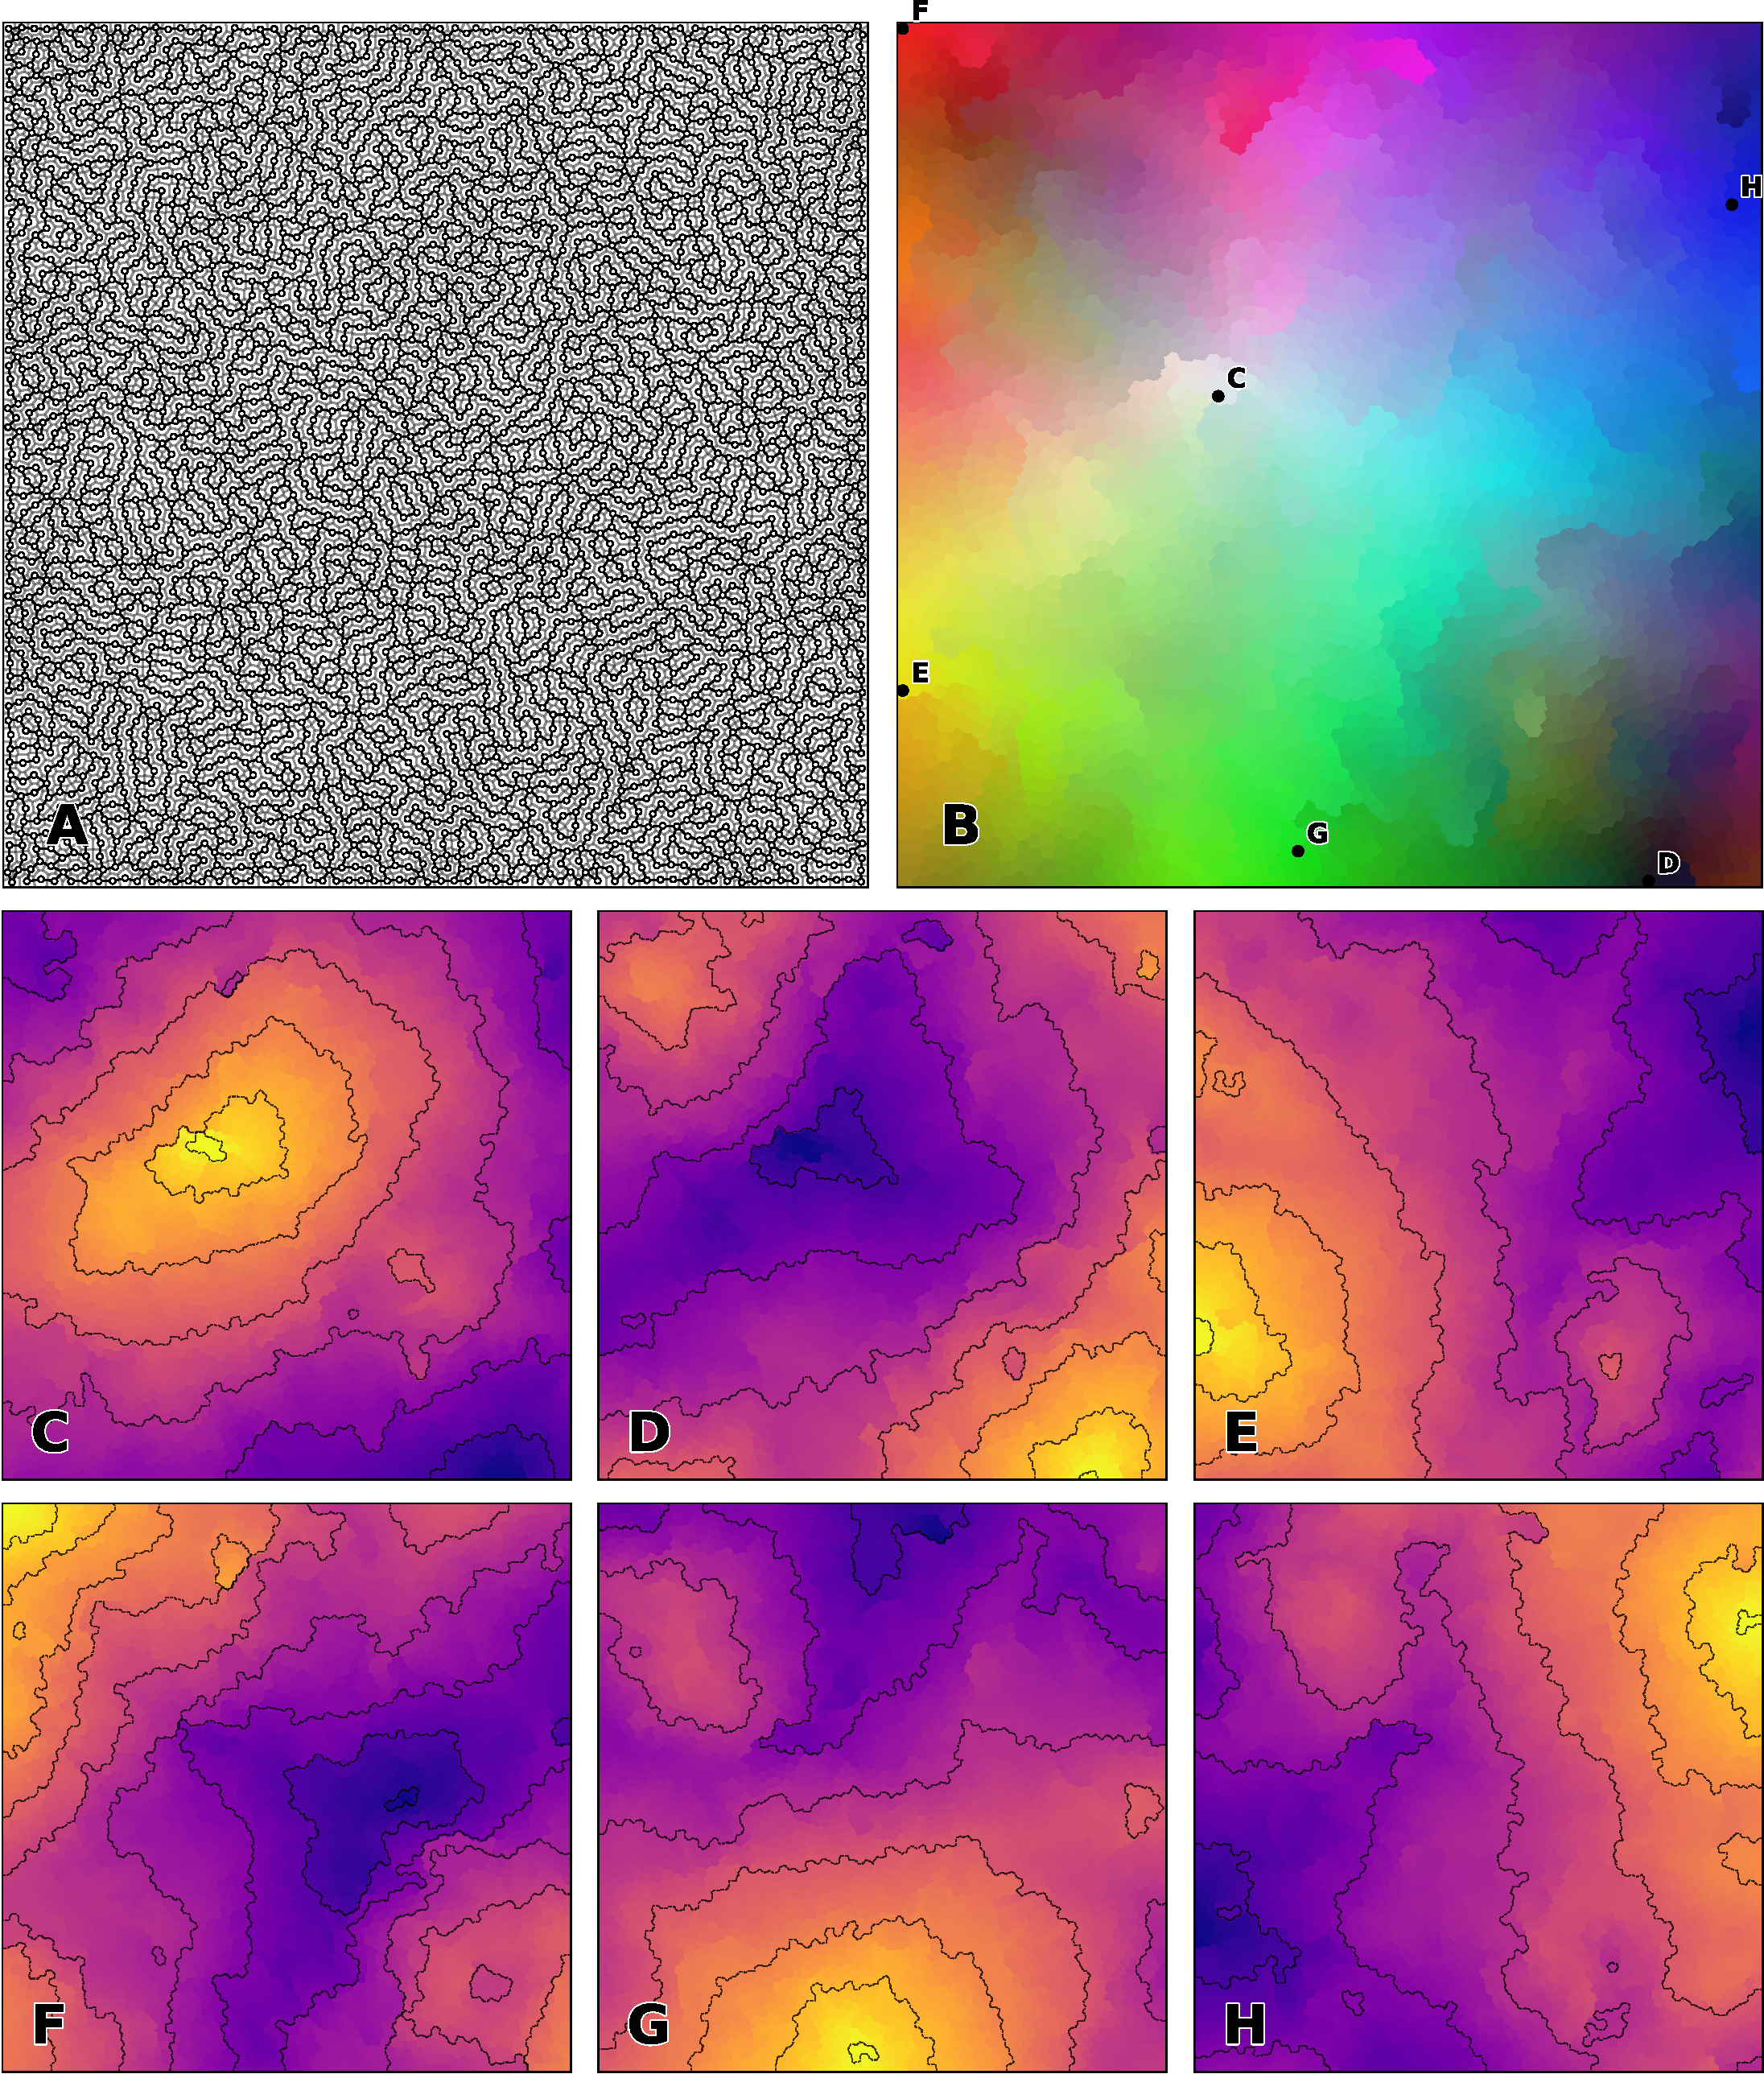
\includegraphics[width=\columnwidth]{experiment-3D-uniform.pdf}
  \vspace{2mm}
  \centering
  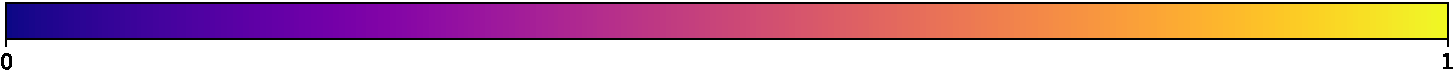
\includegraphics[width=.975\columnwidth]{figures/colormap.pdf}
  %
  \caption{%
  %
  {\bfseries \sffamily Three dimensional uniform dataset (results)}
  %
  Randomized SOM made of $4096$ neurons with a $3$-nearest neighbors induced topology. Model has been trained for $25,000$ epochs on three-dimensional points drawn from a uniform distribution on the unit cube. \textbf{A} Map topology in neural space. \textbf{B} Map codeword in neural space. Each neural voronoi cell is painted with the color of the codeword. \textbf{C to H} Normalized distance map for six samples, respectively (1,1,1), (0,0,0), (1,1,0), (1,0,0), (0,1,0) and (0,0,1) in RGB notations. Normalization has been performed for each sample in order to enhance contrast but this prevents comparison between maps.
  %
  }
  \label{fig:3D-uniform:results}
\end{figure}

\begin{figure}
     \centering
     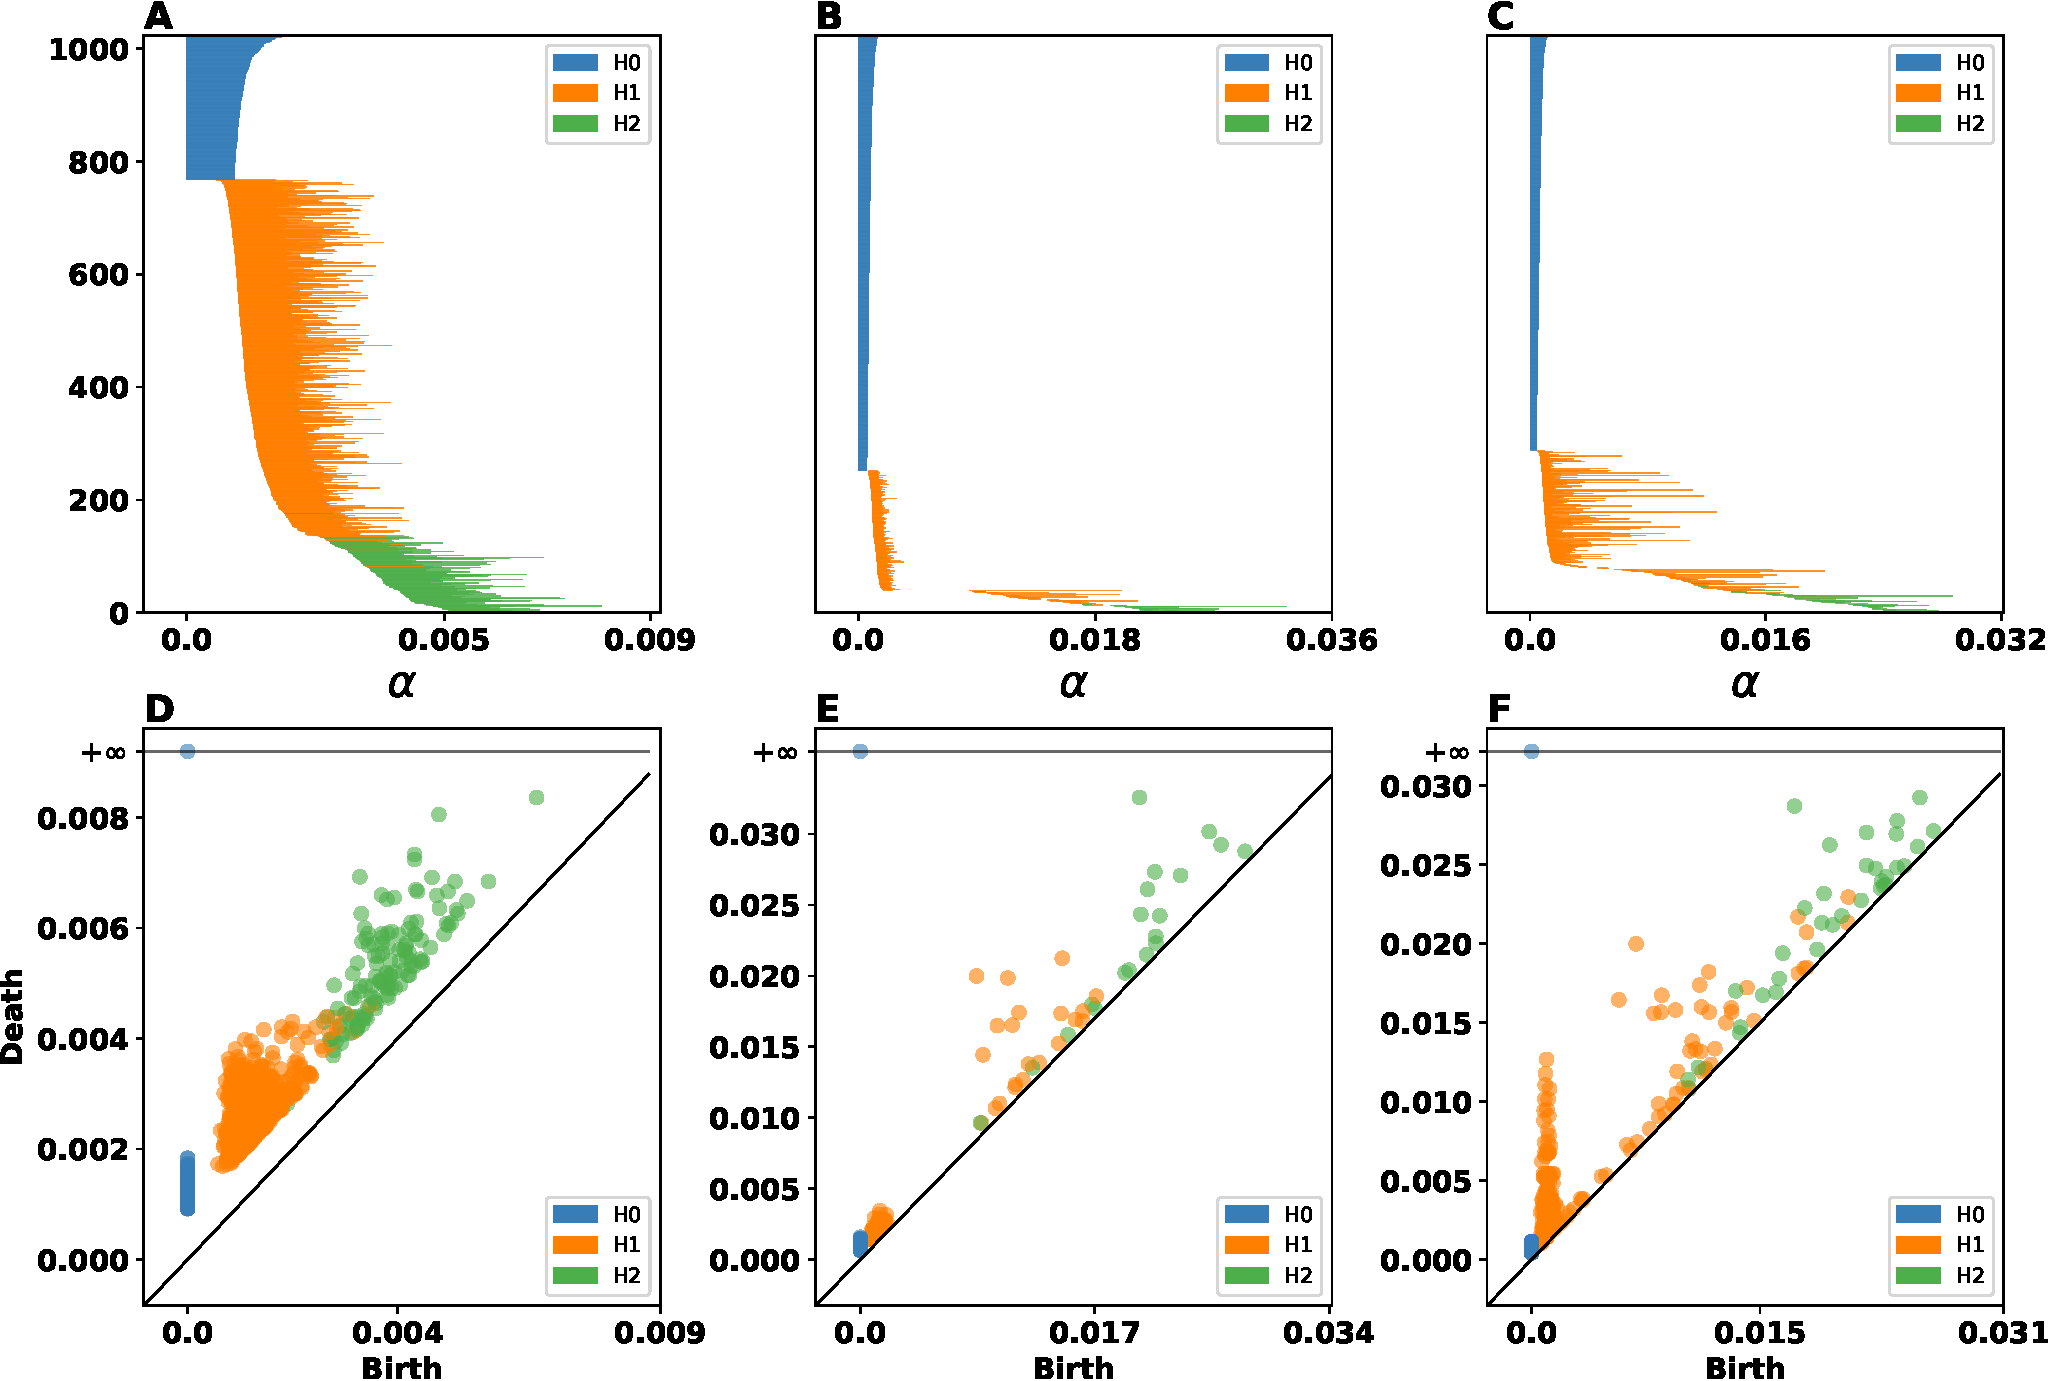
\includegraphics[width=\textwidth]{figures/experiment-3D-uniform-analysis.pdf}
     \caption{ {\bfseries \sffamily Three dimensional uniform dataset (analysis)}
     Persistent Barcodes of \textbf{A} input space, \textbf{B} SOM, and \textbf{RSOM}.
  The blue, orange, and green line segments represent the $H0$-, $H1$-, and $H2$-homology, respectively.
  This means that blue color represents connected segments within the space and orange color reflects the holes
  within the space and the green one the voids. The longer the line segment the more important the 
  corresponding topological feature. \textbf{D} illustrates the persistent diagram for the input space.
  \textbf{E} and \textbf{F} depict the persistent diagrams for SOM and RSOM, respectively. Again blue dots
  indicate $H0$-homology features, orange dots represent $H1$-homolocical features, and green the 
  $H2$-homological features.}
 \label{fig:3D-uniform:analysis}
\end{figure}
